\subsubsection{Referencespænding}\label{Spaendingsref}
\textbf{Teori og design}\\
Der skal ved offset- og komparatorblokken forsynes med en konstant spænding, da spændingen skal anvendes som sammenligningsgrundlag ift. andre signaler. Denne spænding kaldes en referencespænding. Referencespændingen består af en spændingsforsyning, en modstand og en spændingsreference diode. Der anvendes en referencediode af typen LM385, som både findes som $1.2$V og $2.5$V. Et eksempel på en opsætning af en spændingsreference kan ses på figur \figref{fig:Spaendingsreference}.

\begin{figure}[H]
	\centering
	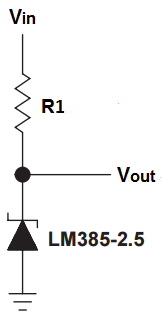
\includegraphics[scale=1.0]{figures/cProblemloesning/ReferenceEksempel.PNG}
	\caption{Figuren illustrerer et eksempel på opsætning af et kredsløb for en spændingsreference med LM$385$. Figuren er en revideret udgave fra kilden. \cite{Instruments2005}}
	\label{fig:Spaendingsreference}
\end{figure}

For at udregne værdien af modstanden, R, i kredsløbet, anvendes følgende generelle formel:
\begin{equation}
R=\dfrac{V_{forsyning}-V_{Reference}}{I_{Z}}
\end{equation}
Hvor $V_{forsyning}$ er forsyningsspændingen som sendes ind i kredsløbet, $V_{Reference}$ er den referencespænding der skal sendes ud af systemet og $I_{Z}$ er strøm forbruget fra de komponenter, der er i referencespændings kredsløbet. 
\noindent \textbf{Beregning af referenceværdien til offset}
Først udregnes R for referencespændingen til offsettet. $V_{forsyning}$ er de $5.5$V, der forsynes med fra spændingsforsyningen. $V_{Reference}$ $2.5$V. I kredsløbet for ofsettet indgår én operationsforstærker (TL$081$), der har en maksimal biasstrøm på $10$nA\cite{Corporation1995}. Referencedioden har et arbejdsområde mellem $20\mu$A til $20mA$ og for at sikre der er strøm nok til referencedioden er den sat til at bruge $200\mu$A \cite{Instruments2005}. Dermed kan strømforbruget, $I_{Z}$, for offsettet udregnes som summen af de to biasstrømme og alle de kendte værdier indsættes i formlen:

\begin{equation}
R_{offset}=\frac{5.5V-2.5V}{0.0002 + (1 \cdot 10^(-8)A} = 14999.25004\Omega \approx 15K\Omega
\end{equation}  
Da offsettet på accelerometeret er på $1.6325$V jævnført \ref{Offset_Teori_Design} på side \pageref{Offset_Teori_Design} skal referenceværdi være ligeledes $1.6325$V. For at opnå denne referenceværdi, bruges der en spændingsdeler. Den genelle formel for spændingsdeler er: 

\begin{equation} \label{Spaendingsdeler}
V_{out}=V_{in}*\dfrac{R2}{R1+R2}
\end{equation}

R$1$ bliver valgt til at være $10$K$\Omega$ og derved er følgende kendt: 
\begin{itemize}
\item $V_{out}$  = $1.6325$V
\item $V_{in}$ = $2.5$V
\item R1 = $10$K$\Omega$
\end{itemize}
Ligningen kommer til at være således: 
\begin{equation}
1.6325V = 2.5* \dfrac{R2}{10000\Omega+R2} 
R2 = 18818.44380\Omega \approx 18820\Omega
\end{equation}

\noindent \textbf{Beregning af referenceværdien til komparator}
Den samme fremgangsmåde anvendes til udregning af R for referencespændingen til komparatoren. Her er den ønskede referenceværdi  $2.5$V, så der benyttes ikke en spændingsdeler. Der er i begyndelse at kredsløbet indsat en operations forstærker (TL$082$), som har to input og output og derved kan fungere som både buffer til komparator kredsløbet og inverterende forstærker. Da spændingsdeleren går direkte ind i en buffer, så er den maksimale biasstrøm på $50nA$. Biasstrømmen for referencedioden er igen sat til $200\mu$A. Dermed kan værdierne igen indsættes i formlen og R kan beregnes.

\begin{equation}
R_komparator = \frac{5.5V-2.5V}{0.000200005A} = 14999.62501\Omega \approx 15K\Omega 
\end{equation} 

\textbf{Simulering af spændingsreference til offsetjustering}\\
Der foretages en simulering i LTspice, for at se hvor præcis spændingsreferencen samt spændingsdeleren er. Resultatet af simuleringen kan ses i \tableref{Tab:SpaendingsRef_offset}

\begin{table}[]
\centering
\caption{I tabellen ses resultaterne fra simuleringen i LTspice af spændingsreferencen til offsetjusteringen.}
\label{Tab:SpaendigsRef_offset}
\begin{tabular}{|l|l|l|l|}
\hline
                              & Forventet & Målt & Afvigelse \\ \hline
Input                         & $5.5$V    &   $5.5$V   &   $0\%$         \\ \hline
Output fra spændingsreference & $2.5$V    &  $2.5007$V    &    $0.0280 \%$        \\ \hline
Output fra spændingsdeler     & $1.6325$V &  $1.6330$V     &       $0.0306 \%$     \\ \hline
\end{tabular}
\end{table}

I tabellen fremgår det at der er lav afvigelse mellem det forventede output og det simulerede output. Dette betyder at kredsløbet fungerer teoretisk og det implementeres derfor. På figur \figref{fig:Spaendingsreference_offset} ses simuleringen af spændingsreferencen med spændingdeler. 

\begin{figure}[H]
	\centering
	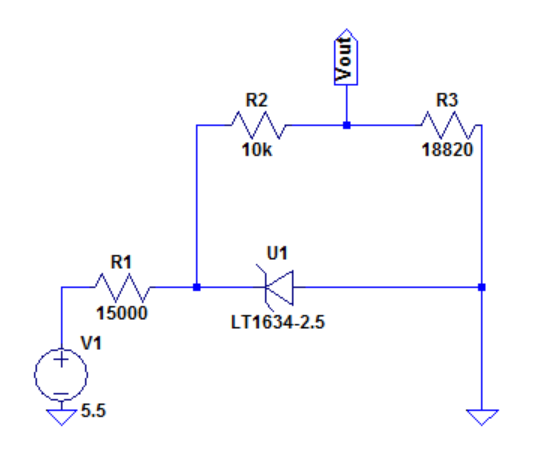
\includegraphics[scale=1.0]{figures/cProblemloesning/OffsetSpaendingsRef.PNG}
	\caption{Opsætning af kredsløbet for en spændingsreference til offsettet. Hvor der først er en spændingsreference efterfølgt at en spændingsdeler, som gør at outputtet fra spændingsreferencen på $2.5$V bliver til $1.6325$V. }
	\label{fig:Spaendingsreference_offset}
\end{figure}

\textbf{Implementering og test af referencespænding til offsetjustering}\\
I implementeringen arbejdes der med reelle komponenter. Derfor antages der, at der kan være afvigelser fra resultaterne imellem testen med ideelle komponenter i dette afsnit og testen med reelle komponenter i simuleringen. \\
Der ses på \figref{fig:Offset_generisk}, at der skal benyttes tre modstande på hhv. $15$K$\Omega$, $10$K$\Omega$ og $18820 \Omega$  til opbygningen af offsettet. Der findes ikke en $18820 \Omega$, derfor benyttes en $18$K$ \Omega$  Disse blev målt inden testen, hvilket fremgår i \tableref{Tab:modstand_offset}.

\begin{table}[H]
	\centering
	\begin{tabular}{|l|l|l|}
		\hline
		\textit{Teoretisk} & \textit{Ved måling} & \textit{\% afvigelse} \\ \hline
		$15$K$\Omega$       & $15002\Omega$       & $0.013$\%               \\ \hline
		$10$K$\Omega$       & $10003.6\Omega$       & $0.036$\%               \\ \hline
		$18$K$\Omega$       & $17966.3 \Omega$       & $0.187$\%               \\ \hline
		$820 \Omega$       & $818.08 \Omega$       & $0.234$\%               \\ \hline
	\end{tabular}
	\caption{I tabellen ses der, at alle fire modstande afviger lidt fra deres teoretiske værdi, hvilket er forventet af reelle komponenter. Kravet til disse fire modstande var dog, at de skulle være ens således at der ikke sker en forstærkning. Disse modstande accepteres derfor.}
	\label{Tab:modstand_offset}
\end{table}

Herefter implementeres kredsløbet. Til aflæsning af spændingsniveauerne anvendes et multimeter. De aflæste resultater står i \tableref{Tab:SpaendingsRef_offset_test}.
\begin{table}[]
\centering
\caption{I tabellen ses en oversigt over de forventede og målte signaler af testen for spændingsreferencen til offsetjustering.}
\label{Tab:SpaendingsRef_offset_test}
\begin{tabular}{|l|l|l|l|}
\hline
                              & Forventet & Målt      & Afvigelse \\ \hline
Input                         & $5.5$V    & $5.550$V  & $0.91 \%$ \\ \hline
Output fra spændingsreference & $2.5$V    & $2.499$V  & $0.04 \%$ \\ \hline
Output fra spændingsdeler     & $1.6325$V & $1.6296$V & $0.18 \%$ \\ \hline
\end{tabular}
\end{table}

Ud fra \tableref{Tab:SpaendingsRef_offset_test} ses det at afvigelserne for inputtet til spændingsreferencen har en lidt større afvigelse end de andre. Dette kan skyldes at spændingsforsyningen ikke er ideel og derfor vil svinge lidt i dens outputspænding. Svingningen fra spændingsforsyningen vil ikke have en indflydelse hvis den ikke svinger mere end det målte. Outputtet fra spændingsreferencen accepteres da afvigelsen er på $0.04 \%$. Det samme gælder for outputtet af spændingsdeleren, hvor afvigelsen er på $0.18 \%$.





 